\documentclass[11pt, brazil]{beamer}
\mode<presentation> {
\usetheme{natali}
\definecolor{crimson}{HTML}{a30000}
\setbeamertemplate{itemize item}{\color{crimson}$\blacksquare$}
\setbeamertemplate{enumerate item}{\color{crimson}$\bullet$}
\setbeamertemplate{caption}[numbered]
\setbeamercolor{section number projected}{bg=crimson,fg=white}
\setbeamercolor{subsection number projected}{bg=crimson,fg=white}
\setbeamercolor{caption name}{fg=crimson}
\setbeamercovered{transparent}
}

\definecolor{darkgreen}{HTML}{008800}
\definecolor{lightgreen}{HTML}{00bb00}
%Mudando a cor do block
\newenvironment{variableblock}[3]{%
 \setbeamercolor{block body}{#2}
 \setbeamercolor{block title}{#3}
\begin{block}{#1}}{\end{block}}
%%%%%%%%%%%%%%%%%%%%%%%%

\setbeamertemplate{navigation symbols}{}
\usepackage[utf8]{inputenc}
\usepackage[brazil]{babel}
\usepackage{graphicx}
\usepackage{booktabs}
\usepackage{array}
\usepackage{amsmath}
\usepackage[customcolors]{hf-tikz}
\usepackage{hyperref}
\usepackage{ragged2e}
\usepackage{libertine}
\usepackage{tabularx}
\usepackage{lscape}
\usepackage{graphicx}% Inclusão de gráficos
\usepackage{microtype} % para melhorias de justificação
\usepackage{amsmath} % Fonte matemática
\usepackage{amssymb} % Fonte matemática
\usepackage{mathrsfs} % Fontes formais matemáticas. Comando: \mathscr{}
\usepackage{bbm} % Fontes formais em matematica para conjuntos (naturais, reais, etc). Comando: \mathbbm{}
\usepackage{latexsym} % Para símbolos matemáticos
\usepackage{multicol}% Suporte a mesclagens em colunas
\usepackage{multirow}% Suporte a mesclagens em linhas
\usepackage{colortbl}
\usepackage{makecell}%Para pular linha da tabela quando tiver texto grande
    
%---------------------------------------------------

\title[Introdução à relatividade]{\bf {\small XIX Semana da Física:}\\
 Minicurso: Introdução à relatividade}
\author[natalidesanti@gmail.com]{{\bf Natalí Soler Matubaro de Santi}\\
       \texttt{\footnotesize natalidesanti@gmail.com}}
\vspace{0.7cm}
\institute[DF/UNESP]{Departamento de Física\\
 Universidade Estadual Paulista Júlio de Mesquita Filho}
\vspace{0.7cm}
\date{20 de Setembro de 2019}

\begin{document}
\setbeamercovered{invisible}

\begin{frame}
 \titlepage 
\end{frame}

%------------------------------------------------

\begin{frame}
\frametitle{Prêmios}
\begin{enumerate}
 \justifying
 \item {\color{crimson}\bf Nobel} (1901 - hoje): 590 prêmios para 935 laureados
  \begin{itemize}
   \justifying
   \item 51 mulheres;
   \item 3 físicas:
     \begin{enumerate}
       \item 1903: {\color{crimson}\bf Marie Sklodowska Curie} - fenômeno da radiação;
       \item 1963: {\color{crimson}\bf Maria Goeppert-Mayer} - estrutura das camadas nucleares;
       \item 2018: {\color{crimson}\bf Donna Strickland} - pulsos ópticos ultracurtos de alta intensidade;
     \end{enumerate}
  \end{itemize}
 \pause  
 \item {\color{crimson}\bf Wolf - Física} (1978 - hoje): 31 prêmios para 61 laureados
  \begin{itemize}
   \justifying
   \item 1 mulher:
     \begin{enumerate}
       \item 1978: {\color{crimson}\bf Chien-Shiung Wu} - não conservação da paridade na interação fraca;
     \end{enumerate}
  \end{itemize}
 \pause  
 \item {\color{crimson}\bf Einstein} (2003 - hoje): 11 prêmios para 11 laureados
  \begin{itemize}
   \justifying
  \item Nenhuma mulher;
 \end{itemize}     
\end{enumerate}
\vspace{-0.1cm}
\begin{figure}
 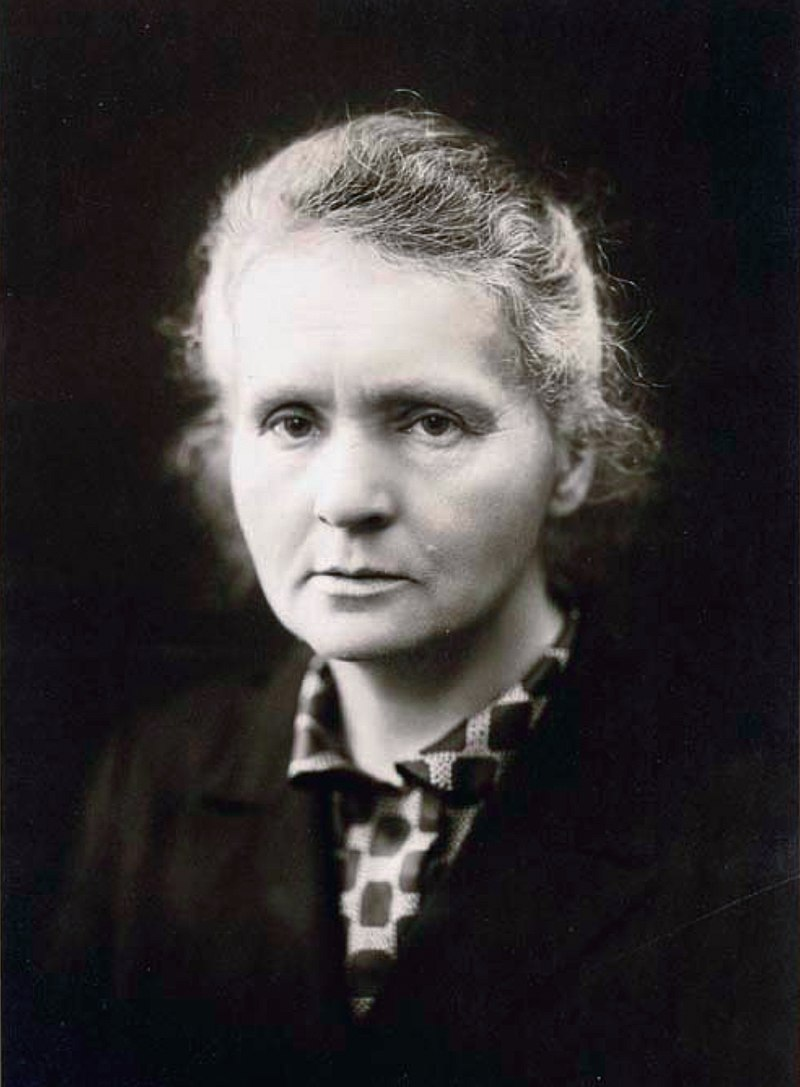
\includegraphics[scale=0.06]{figuras/curie.jpg}
 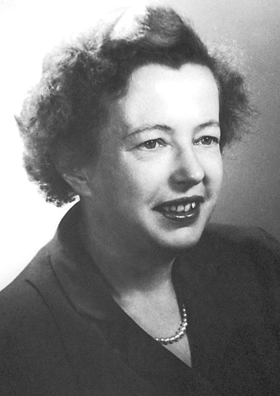
\includegraphics[scale=0.17]{figuras/mayer.jpg}
 
\includegraphics[scale=0.084]{figuras/donna.jpg}
 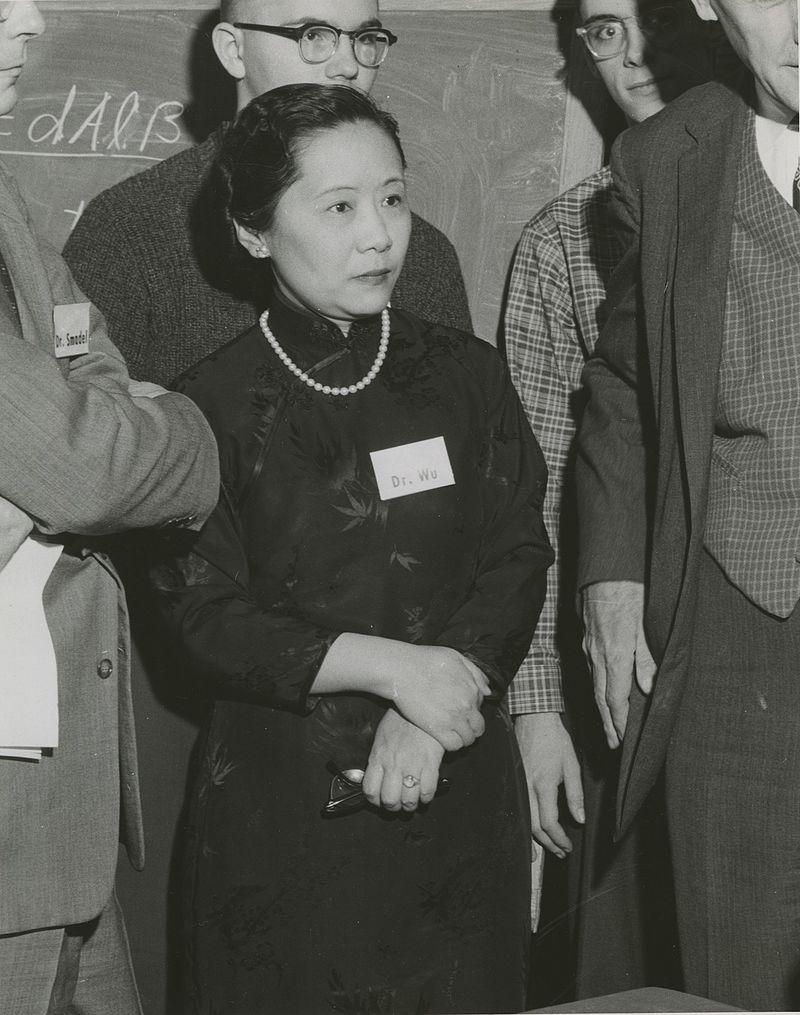
\includegraphics[scale=0.65]{figuras/chien.jpg}
\end{figure}  
\end{frame}

%------------------------------------------------

\begin{frame}
\frametitle{Relativísticas}
\begin{columns}
\column{0.7\textwidth}
\begin{enumerate}
 \justifying
 \item {\color{crimson}\bf Emmy Noether} (1882 - 1935):
  \begin{itemize}
   \justifying
   \item Matemática;
   \item Seu principal teorema em Física explica a conexão entre as simetria e as leis de conservação.
  \end{itemize}
\end{enumerate}
\column{0.3\textwidth}
\begin{figure}
 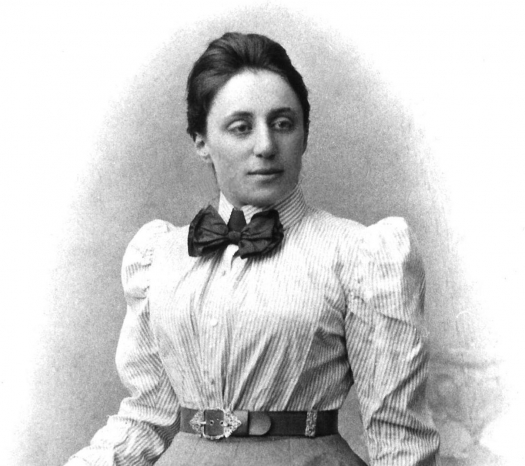
\includegraphics[scale=0.15]{figuras/noether.jpg}
\end{figure}
\end{columns}
\pause  
\begin{columns}
\column{0.7\textwidth}
\begin{enumerate}
 \justifying
 \item {\color{crimson}\bf Mileva Maric} (1875 - 1948):
  \begin{itemize}
   \justifying
   \item Matemática;
   \item Segunda mulher a completar seus estudos no Departamento de Física e Matemática da universidade de Zurich;
   \item Primeira esposa de Albert Einstein - divórcio em 1919;
   \item ``Profunda influência'' nos trabalhos de Einstein.  
  \end{itemize}
\end{enumerate}
\column{0.3\textwidth}
\begin{figure}
 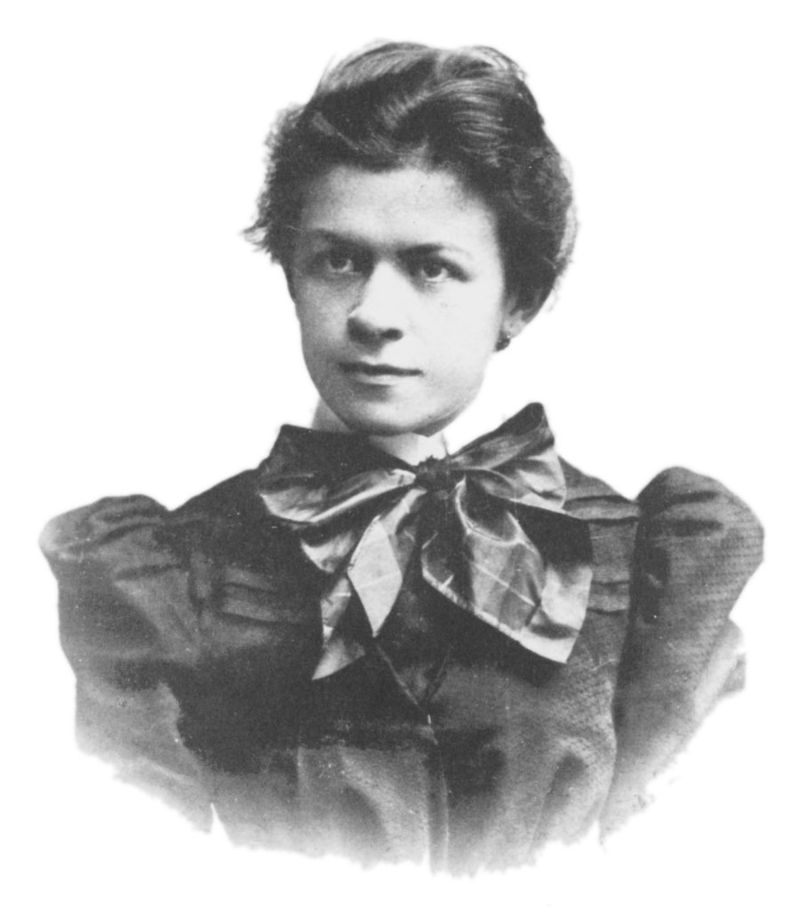
\includegraphics[scale=0.37]{figuras/mileva.jpg}
\end{figure}
\end{columns}
\end{frame}

%------------------------------------------------

\begin{frame}
\frametitle{Computeiras}
\begin{columns}
\column{0.7\textwidth}
\begin{enumerate}
 \justifying
 \item {\color{crimson}\bf Margaret Hamilton} (1936 - hoje):
  \begin{itemize}
   \justifying
   \item Cientista da Computação;
   \item Diretora da divisão de engenharia de software responsável pelas missões Apolo;
  \end{itemize}
\end{enumerate}
\column{0.3\textwidth}
\begin{figure}
 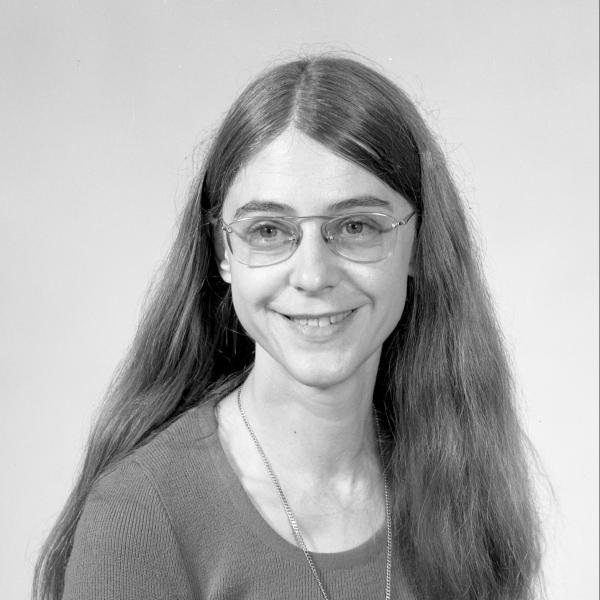
\includegraphics[scale=0.13]{figuras/hamilton.jpg}
\end{figure}
\end{columns}
\pause  
\begin{columns}
\column{0.7\textwidth}
\begin{enumerate}
 \justifying
 \item {\color{crimson}\bf Katie Bouman} (1889 - hoje):
  \begin{itemize}
   \justifying
   \item Cientista da Computação;
   \item Desenvolvedora do algoritmo {\em Continuous High-resolution Image Reconstruction using Patch priors (CHIRP)};
   \item Responsável pela obtenção da {\bf primeira imagem de um buraco negro} (Junho de 2019);
   \item Membro do {\em Event Horizon Telescope (EHT)}.  
  \end{itemize}
\end{enumerate}
\column{0.3\textwidth}
\begin{figure}
 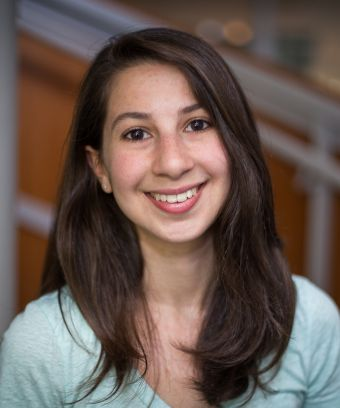
\includegraphics[scale=0.3]{figuras/katie.jpg}
\end{figure}
\end{columns}
\end{frame}

%------------------------------------------------

\begin{frame}
\frametitle{Sobre mim}
\begin{enumerate}
 \justifying
 \item Sou física teórica; 
 \item Bacharela em física pela USP em 2015;
 \item Mestra em física pela UFSCar em 2018;
 \item Realizo meu doutorado em física pela USP;
\end{enumerate}
\pause  
\begin{figure}
 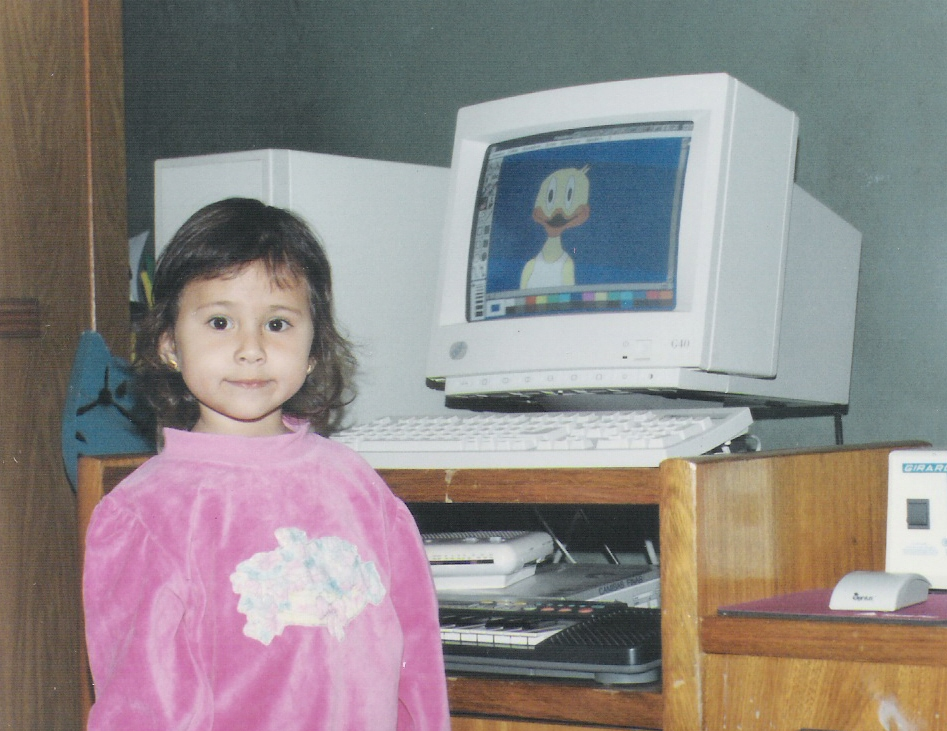
\includegraphics[scale=0.4]{figuras/comp.jpg}
 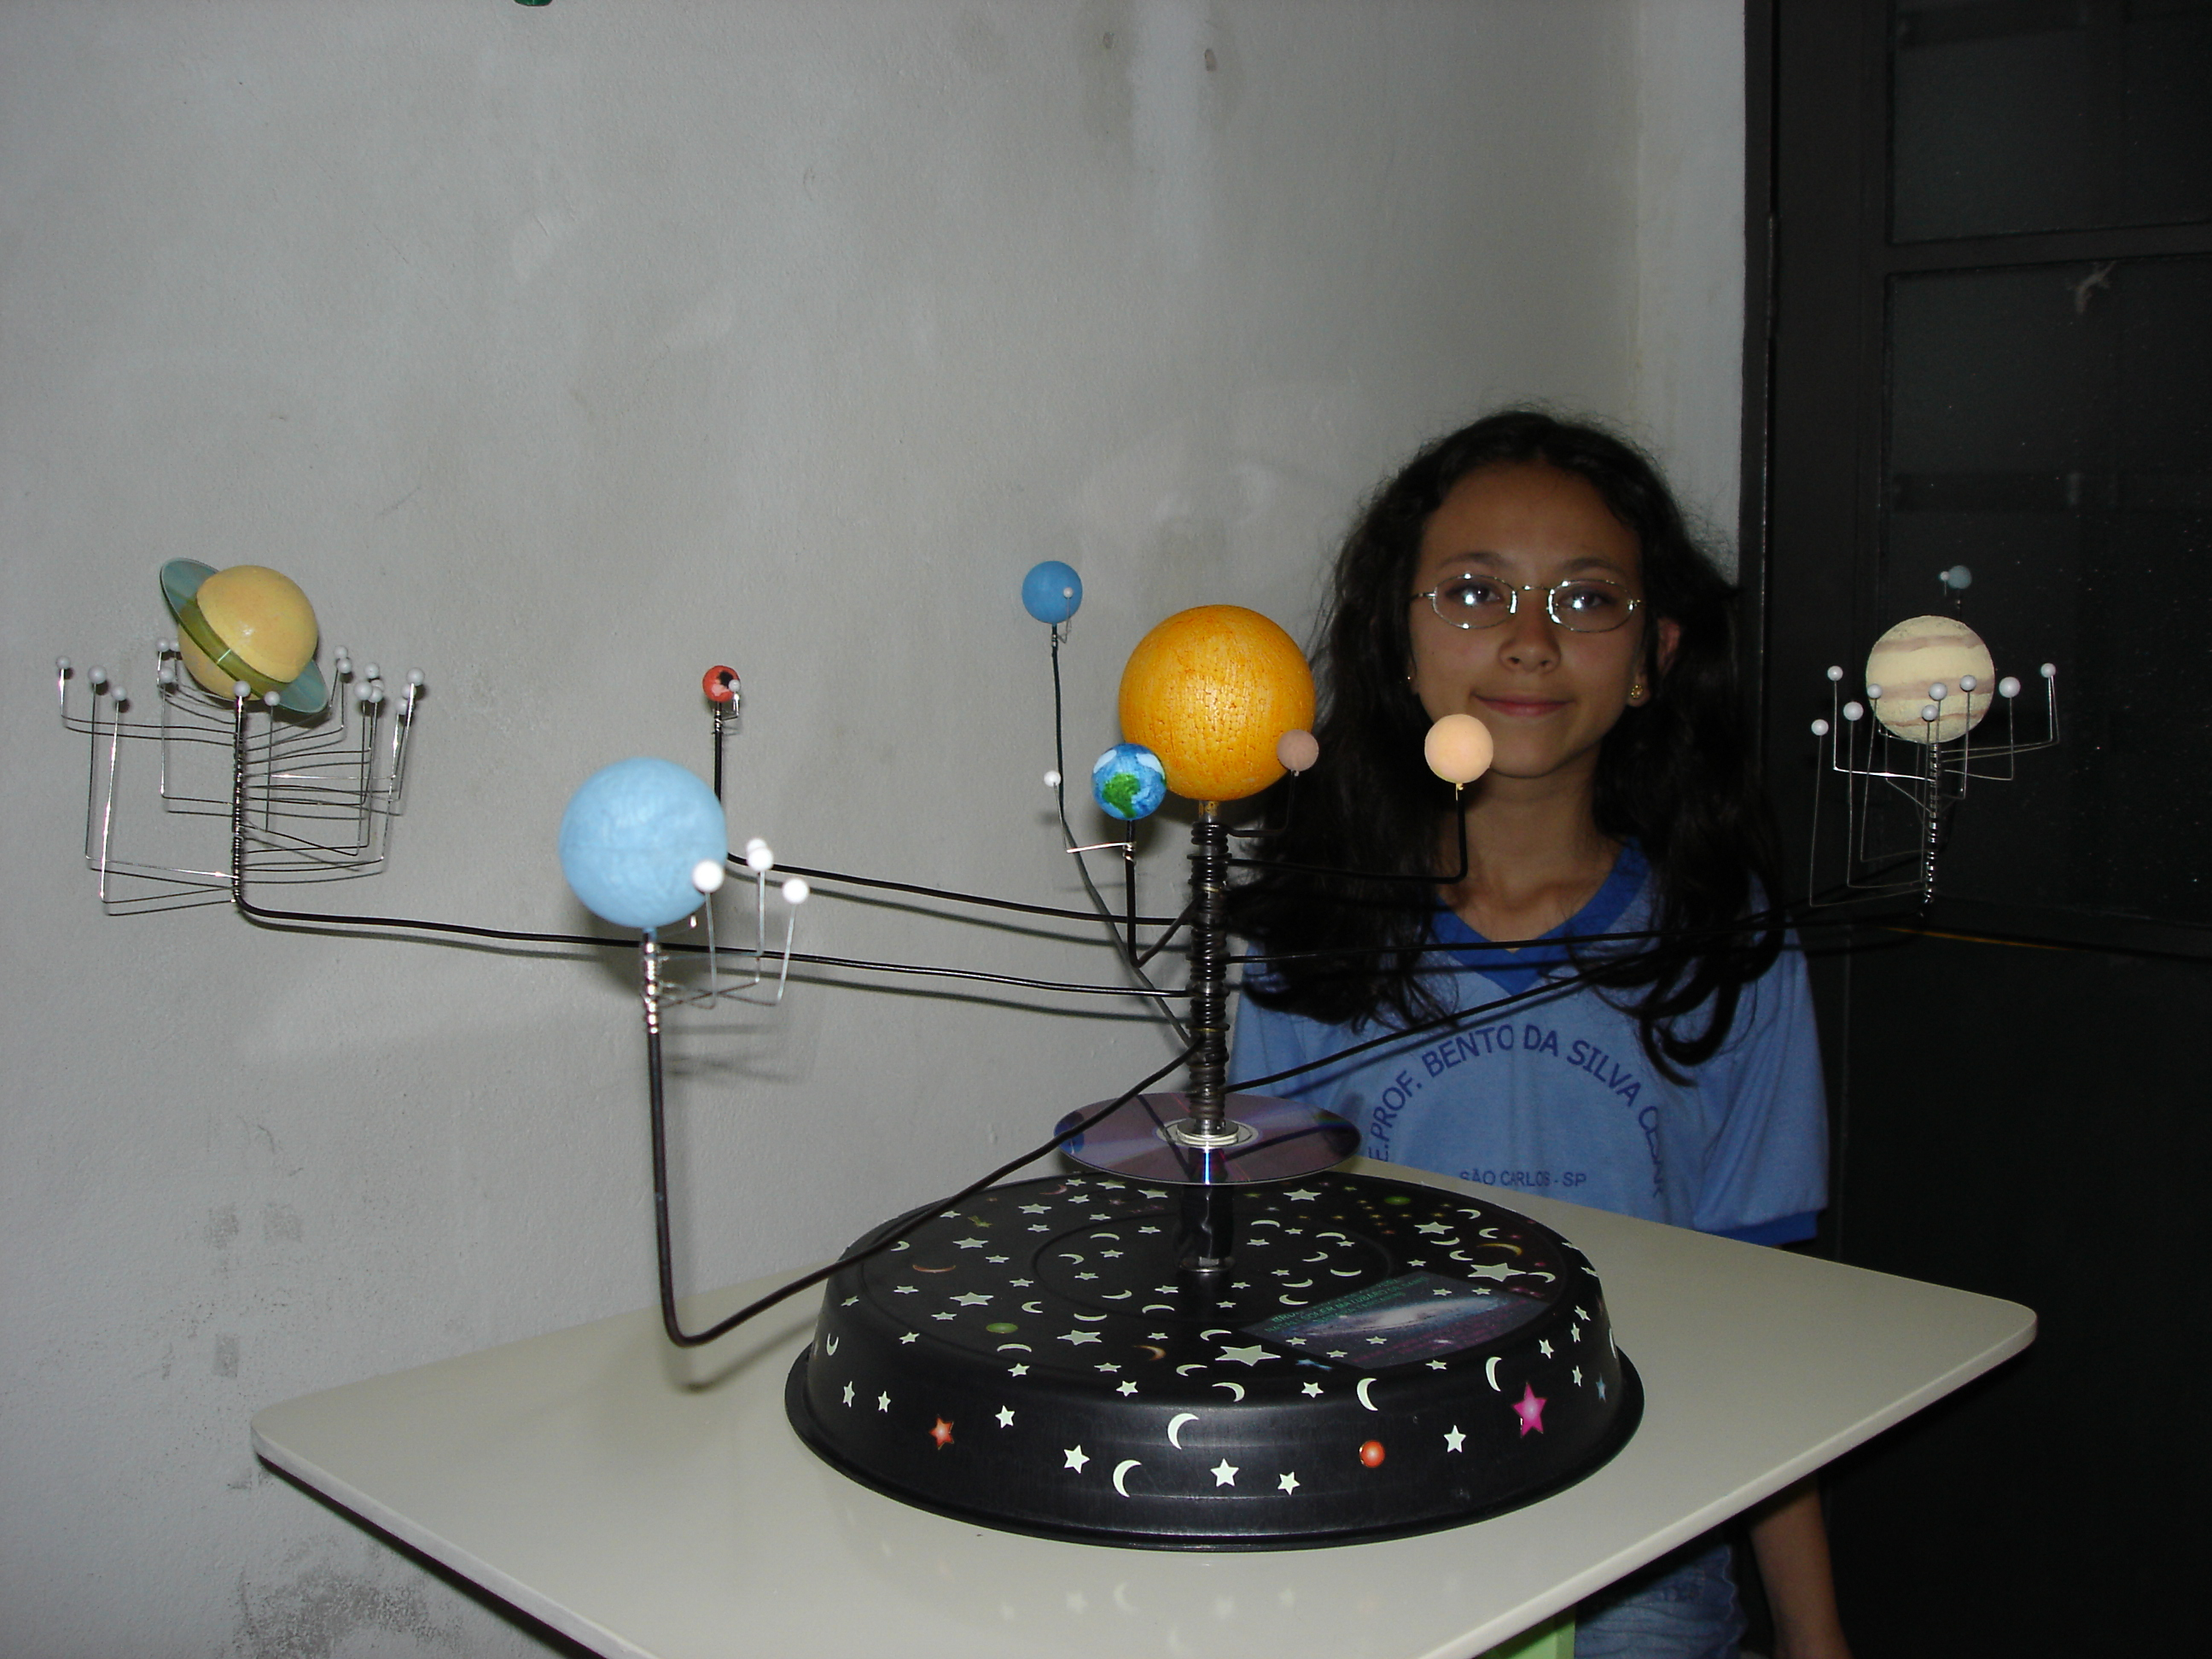
\includegraphics[scale=0.054]{figuras/solar.jpg}
\end{figure}  
\end{frame}

%------------------------------------------------

\begin{frame}
\frametitle{Sobre vocês}
\begin{enumerate}
 \justifying
 \item Agora é a sua vez: 
\end{enumerate}
\begin{figure}
 
\includegraphics[scale=0.5]{figuras/u.jpeg}
\end{figure}  
\end{frame}


%------------------------------------------------

\begin{frame}
\frametitle{Objetivos do minicurso}
\begin{enumerate}
 \justifying
 \item Princípios básicos da {\color{crimson}\bf teoria da relatividade}:
  \begin{itemize}
   \justifying
   \item Notação covariante;
   \item Terminologia da dinâmica relativística; 
  \end{itemize}
 \pause  
 \item {\color{crimson}\bf Relatividade especial (RE):}
  \begin{itemize}
   \justifying
  \item Transformações de Lorentz;
  \item Contração espacial;
  \item Dilatação temporal;
  \item Conservação de energia e momentum;  
 \end{itemize}     
 \pause  
 \item {\color{crimson}\bf Relatividade geral (RG):}
  \begin{itemize}
   \justifying
  \item Conceito de espaço-tempo curvo;
  \item Tensor de Riemann, Ricci e escalar de Ricci;
  \item Equações de Einstein;
  \item A solução de Schwarzschild.
 \end{itemize}     
\end{enumerate}  
\end{frame}

%------------------------------------------------

\end{document}

%%% Local Variables:
%%% mode: latex
%%% TeX-master: t
%%% End:
